\documentclass[11pt]{article}
\usepackage[left=0.7in,right=0.7in,top=1in,bottom=0.7in]{geometry}
\usepackage{fancyhdr} % for header
\usepackage{graphicx} % for figures
\usepackage{amsmath}  % for extended math markup
\usepackage{amssymb}  % "" (more math symbols)
\usepackage[bookmarks=false]{hyperref} % for URL embedding
\usepackage[noend]{algpseudocode} % for pseudocode
\usepackage[plain]{algorithm} % float environment for algorithms
\usepackage{float}
\usepackage{mhchem}
\usepackage{xurl}
\usepackage{multirow}
\usepackage{CJKutf8}
\newcommand{\cn}[1]{\begin{CJK*}{UTF8}{gbsn}#1\end{CJK*}}
\usepackage[style=apa,backend=biber]{biblatex}
\defbibheading{centeredbib}[\bibname]{%
  \section*{\centering #1}%
  \markboth{#1}{#1}}
\addbibresource{complit-4320.bib}


%%%%%%%%%%%%%%%%%%%%%%%%%%%%%%%%%%%%%%%%%%%%%%%%%%%%%%%%%%%%%%%%%%%%%%
% STUDENT: modify the following fields to reflect your
% name/WUSTL Key, the current lab (module), and the current problem number

% Example: 
%\newcommand{\StudentName}{Jeremy Buhler}
%\newcommand{\WUSTLKey}{jbuhler}

\newcommand{\StudentName}{Charlie Li}
\newcommand{\StudentID}{518340}

%%%%%%%%%%%%%%%%%%%%%%%%%%%%%%%%%%%%%%%%%%%%%%%%%%%%%%%%%%%%%%%%%%%%%%%%
% You can pretty much leave the stuff up to the next line of %%'s alone.

% create header and footer for every page
\pagestyle{fancy}
\fancyhf{}
\lhead{\textbf{\StudentName}}
\chead{\textbf{\StudentID}}
\rhead{}
\cfoot{\thepage}

% preferred pseudocode style
\algrenewcommand{\algorithmicprocedure}{}
\algrenewcommand{\algorithmicthen}{}

% ``do { ... } while (cond)''
\algdef{SE}[DOWHILE]{Do}{doWhile}{\algorithmicdo}[1]{\algorithmicwhile\ #1}%

% ``for (x in y ... z)''
\newcommand{\ForRange}[3]{\For{#1 \textbf{in} #2 \ \ldots \ #3}}

% these are common math formatting commands that aren't defined by default
\newcommand{\union}{\cup}
\newcommand{\isect}{\cap}
\newcommand{\ceil}[1]{\ensuremath \left\lceil #1 \right\rceil}
\newcommand{\floor}[1]{\ensuremath \left\lfloor #1 \right\rfloor}

%%%%%%%%%%%%%%%%%%%%%%%%%%%%%%%%%%%%%%%%%%%%%%%%%%%%%%%%%%%%%%%%%%%%%%

\title{Post-COVID Trust in Traditional Chinese Medicine(TCM): A Comparative Opinion Mining Study}
\author{Charlie Li}
\date{\today}
\begin{document}
\maketitle

1. Introduction (hypothesis, summary of data, methods and results)
2. Hypothesis (explain reasoning behind hypothesis)
3. Data (describe and defend your dataset, as well as how you compiled it)
4. Method (describe and defend your methodology)
5. Analysis with visualizations (Represent the relevant parts of your results using effective
visualizations appropriate to the method and research question)
6. Results (Summarize findings and how they adhere to or differ from your hypothesis)
7. Conclusion (explain avenues for further exploration or research based on your findings)

\section{Introduction}

Traditional Chinese Medicine (TCM) employs acupuncture and herbal decoctions, among other methods, to treat diseases holistically with an aim to restore balance of the human system. In China, TCM was widely prescribed during the pandemic of COVID-19, which led to heated debates on its effectiveness. On the other hand, evidence-based medicine (EBM) is colloquially called “Western Medicine” in Chinese and positioned at the opposite of TCM. However, few studies have directly compared public trust in TCM to that in EBM. Given the profound influences of COVID-19 on people's attitudes toward healthcare and the global trend of opinion polarization in medicine, it is desirable to explore post-pandemic public trust in both forms of medicine.

Social media platforms are vast reservoirs of public opinions, with online anonymity promoting the expression of uncensored thoughts. While social media connect users across geographic locations and facilitates communication, it can also amplify rumors and affect people's decision making, especially in certain healthcare domains like vaccination \parencite{piedrahitavalds_2021_vaccine}. Therefore, monitoring the trend of sentiments on social media is crucial to understanding public opinion towards healthcare and devicing public health interventions.

In this study, we investigate public trust in TCM versus EBM as expressed on social media platforms across three comparative dimensions: relative to each other, temporally (during and post-COVID), and geoculturally (China versus English-speaking countries). We hypothesize a moderately lower but increasing trust in TCM compared to EBM in China and a significantly lower trust in TCM compared to EBM in English-speaking countries, with a stronger preference for TCM in China.


\section{Hypothesis}

Temporally, the extensive use of TCM in China during the pandemic is hypothesized to have a positive effect on public trust in TCM, which is supported by studies on public opinions during COVID. Using sentiment analysis on 215,565 Weibo (the Chinese equivalent of former Twitter or X) posts published from Jan 24, 2020 to Mar 31, 2020, \textcite{gao_2021_weibo} examined public opinions toward TCM during the pandemic and reported 12\% positive emotions as opposed to 10\% negatives. Upon closer examination, they found that many negative emotions are not aimed at TCM and concluded their study with a generally positive attitude towards TCM. Similarly, \textcite{wang_2024_useful} found a generally supportive attitude toward TCM by manually analyzing 1954 responses on Zhihu (the Chinese equivalent of Quora) posted from Dec 1, 2019 to Feb 28, 2023. This positive effect is hypothesized to result in an increased trust in TCM post-COVID in China. TCM in the flu category are closely adjacent to the treatment of COVID and therefore are hypothesized to see a significant increase in public trust in China, while those in the other two categories are likely to see a milder effect. With the large amount of discussions centered around TCM, I further hypothesize a mild spill-over effect by which English-speaking netizens are exposed to TCM online. Despite the scarcity of coverage on TCM in English-speaking countries, this effect is hypothesized to increase public trust in TCM outside of China.

On the other hand, evidence-based medicine (EBM) remains the dominant healthcare choice globally. However, polarization of public opinions have been on the rise. One of the most researched topics in public opinions on EBM is vaccine hesitancy. Using a hybrid approach to sentiment analysis combining machine learning with lexicon-based methods, \textcite{piedrahitavalds_2021_vaccine} mined 1,499,227 English and Spanish Twitter posts on vaccination published from June 1, 2011 to April 30, 2019. They found a decreasing percentage of neutral sentiments with increasing positives and negatives, showing a concerning trend of attitude polarization. It is hard to hypothesize how trust in EBM shifts post-COVID. If anything, it will likely be a mixed effect. I hypothesize that trust in EBM will remain high both in China and English-speaking countries with minor fluctuations.

Given that TCM receives much more attention in China compared to English-speaking countries, public opinions in China, whether positive or negative, are likely to be amplified. Since the effectiveness of TCM has traditionally been under debate, trust in TCM is likely lower than that in EBM. However, given our temporal hypothesis of increasing trust, I expect post-COVID trust in TCM to be close to that in EBM in China. This effect will be milder in English-speaking countries, where I expect the gap between public trust in TCM and EBM to be larger.

The geocultural hypothesis summarizes the temporal and relative effects. Given a larger increase in post-COVID trust in TCM in China compared to that in English-speaking countries, I expect to see a stronger post-COVID preference for (or weaker disfavor of) TCM over EBM in China compared to English-speaking countries.

\section{Data}
My corpus consists of 5232 Reddit posts and 12806 Weibo posts, totaling 18038 posts, published between year 2019 and 2026. This time spans from the pandemic (2019-2023) to post-pandemic (2024-2026) periods, allowing for temporal analyses. Posts are gathered through web scraping: Reddit was scraped using its json API on March 28, 2026, while Weibo was scraped using the open-source software MediaCrawler from April 5 to April 6, 2026.

Since TCM and EBM are vast fields, directly gathering posts mentioning them is likely to result in extremely noisy data. Moreover, while TCM is a neutral phrase in Chinese, EBM ("Western Medicine") is almost exclusively used in debates over TCM in China, and its variants such as "modern medicine" in English similarly carry opinions by themselves. Therefore, searching for posts mentioning EBM is almost guaranteed to skew the results toward polarization. To narrow the focus, I developed a list of medicine names covering three condition categories: flu, diabetes, and eczema. Flu is chosen due to its relevance to COVID. It is an acute condition, while diabetes and eczema are both chronic diseases. Treatments for eczema involve topical creams, while those for flu and diabetes are predominantly oral or injections. Therefore, the choice of conditions maximize coverage of different kinds of medications. Under each category, I picked three common medicines in both TCM and EBM, resulting in a list of 18 medicine names (table \ref{tab:medicine_list}). The list further includes all common variants and commercial names of these medicines. I searched for and filtered posts based on the list of medicine keywords.
\begin{table}[htbp]
    \centering
    \renewcommand{\arraystretch}{1.5}
    \begin{tabular}{|l|l|l|}
        \hline
        \textbf{Condition} & \textbf{Category} & \textbf{Medicine Keywords} \\
        \hline
        \multirow{2}{*}{Flu} & TCM & Lianhua Qingwen, Banlangen, Yinqiao \\ \cline{2-3}
        & EBM & TamiFlu, Ibuprofen, Acetaminophen \\
        \hline
        \multirow{2}{*}{Diabetes} & TCM & Xiaoke Wan, Liuwei Dihuang Wan, Coptis \\ \cline{2-3}
        & EBM & Metformin, Glimepiride, Insulin \\
        \hline
        \multirow{2}{*}{Eczema} & TCM & Phellodendron Liquid, Qingshi Antipruritic Ointment, Danpifen Ruangao \\ \cline{2-3}
        & EBM & Hydrocortisone, Mometasone furoate, Calamine lotion \\
        \hline
    \end{tabular}
    \caption{List of selected medicines by condition and category}
    \label{tab:medicine_list}
\end{table}

Since each post can mention more than one kind of medicine, the data is then pivoted longer by \texttt{note\_id} and \texttt{medicine\_name}, i.e. one \texttt{note\_id} can correspond to multiple entries with different \texttt{medicine\_name}. The language of the posts is then identified by predictive modeling using the \texttt{fasttext} model \parencite{joulin2016bag, joulin2016fasttext}. Only English posts are selected for Reddit, and only Chinese posts are selected for Weibo, with a confidence cutoff of 0.4, which is a less conservative value that preserves more data. Note that Reddit posts can have both a title and a content, which are classified separately. Since contents are usually much longer than titles, the prediction is more accurate for contents, and the decision is made based solely on content predictions whenever it's available. Since TCM names in English are mostly pingyin and can be mis-recognized as non-English, I examined the model confidence for TCM and EBM posts on Reddit that were classified as English. The distribution of confidence is similar for the two medicine types (figure \ref{fig:en_conf}), which shows that the model is not being confused by TCM names.

\begin{figure}[htbp]
    \centering
    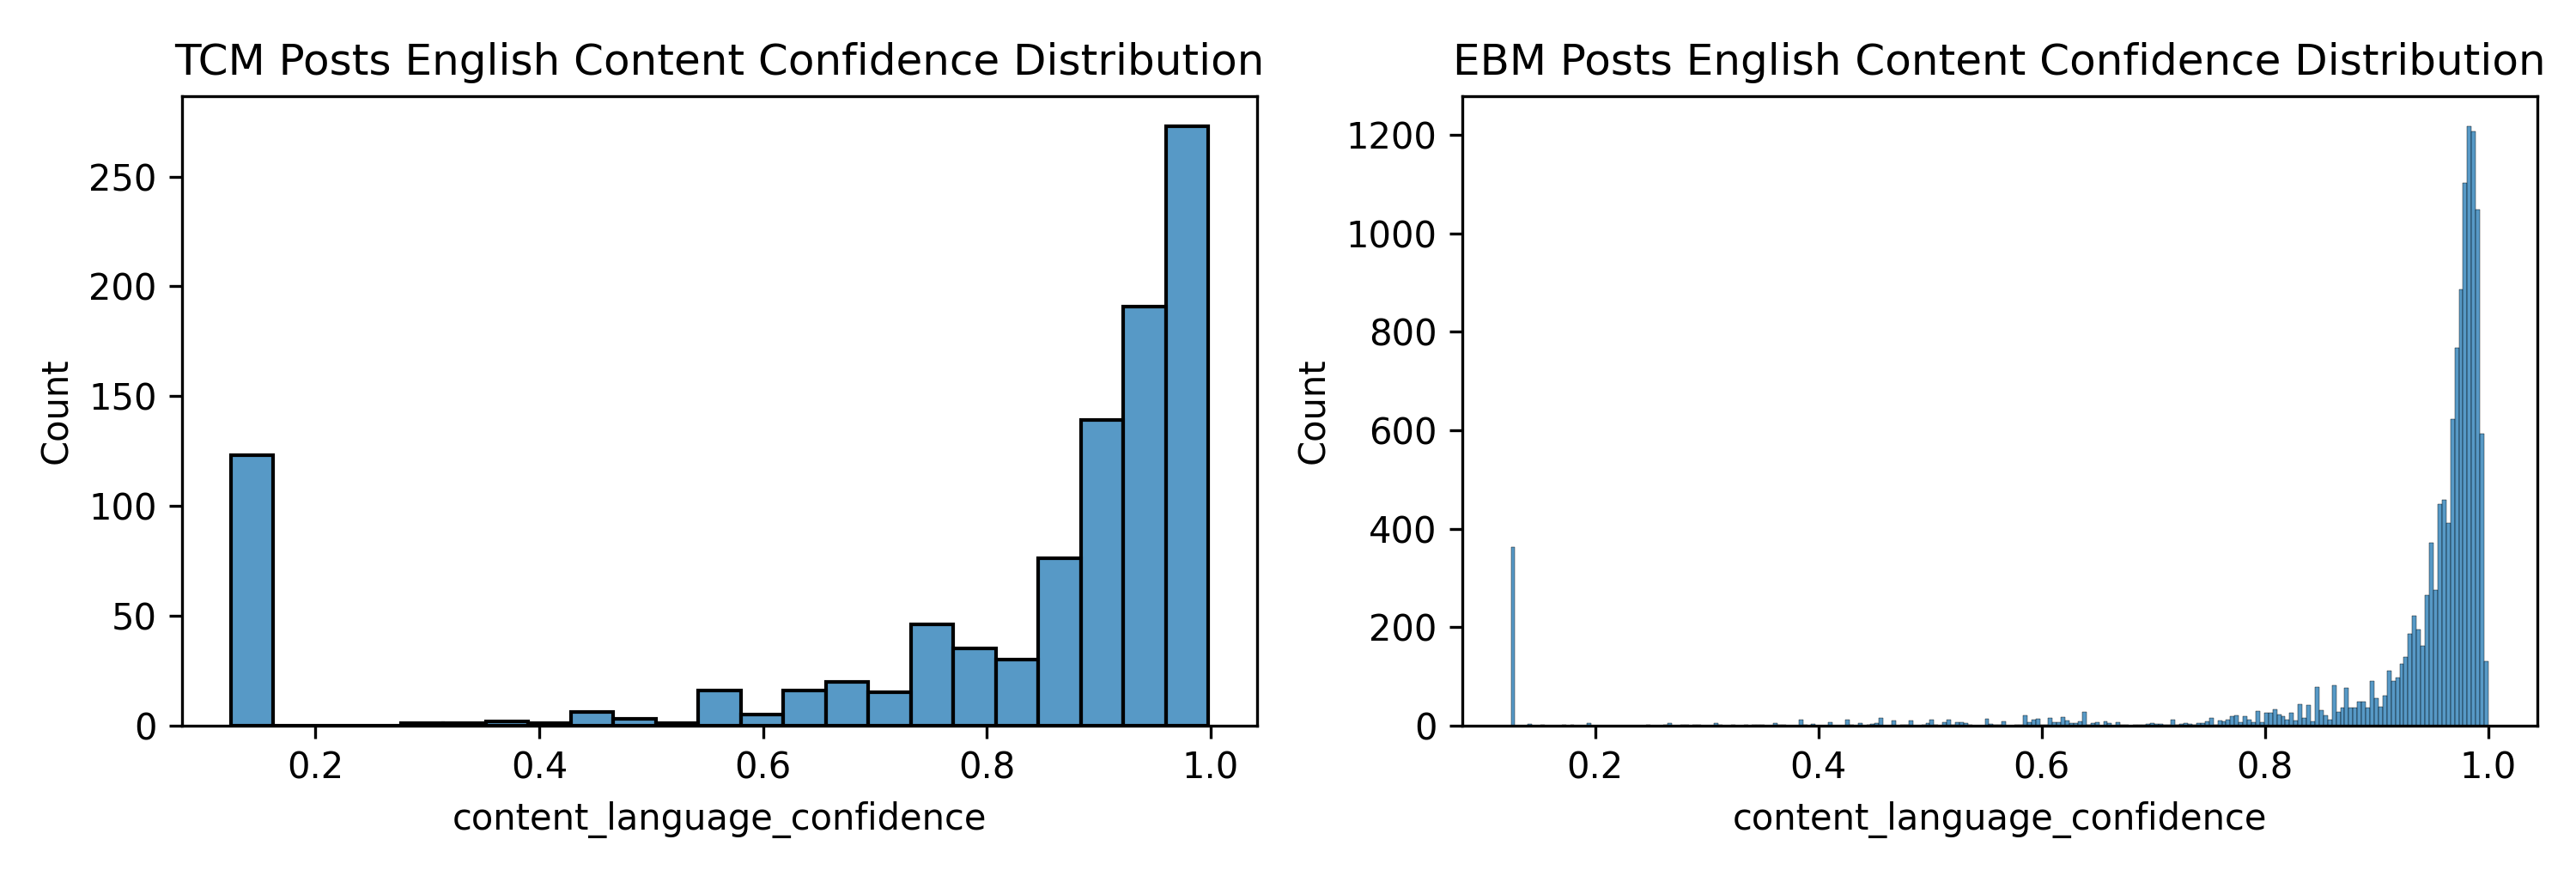
\includegraphics[width=0.8\linewidth, height=0.8\textheight, keepaspectratio]{../../scraping/plots/english_conf_by_med_type.png}
    \caption{Distribution of \texttt{fasttext} prediction confidence for contents of Reddit posts labeled as English, grouped medicine type.}
    \label{fig:en_conf}
\end{figure}

A central assumption of isolation in my study is that Chinese posts on Weibo reflect opinions from Chinese netizens, while English posts on Reddit reflect opinions from English-speaking netizens. This assumption is based on China's Internet censorship with the Great Firewall, which blocks domestic access to certain foreign websites including Reddit \parencite{chan_2011_chinas}. While foreign users are not restricted on Weibo, Chinese posts by English speakers are expected to be rare since Chinese is not a global language. In reality, there are Chinese emmigrant who make active contributions on Reddit, and the use of VPN permits access to Reddit from within the country. These scenarios are expected to account for a minor portion of the posts without skewing the results, although this is debatable for English posts on TCM, which is a rather niche topic in English-speaking countries and may reflect significant input from Chinese netizens.

The final cleaning step is to remove irrelevant posts. While I classified the medicines into three categories, my aim was to explore public opinions on the medicine itself, which does not need to be tied with the specific health condition. Instead, irrelevancy is defined using the following exclusion criteria:
\begin{itemize}
    \item \textbf{Clinical/Physiological Studies (Not Patient Perspective)}
    \item \textbf{Drug Price/Industry/Stock Market}
    \item \textbf{Manufacturing Procedures}
    \item \textbf{Veterinary Cases}
\end{itemize}

I again used predictive modeling to classify the posts as relevant or not. I selected a random sample of 447 posts from the dataset stratified by language, and manually annotated their relevancy. Feature extraction is performed using the pretrained multilingual model \texttt{XLM-RoBERTa} \parencite{DBLP:journals/corr/abs-1911-02116}, and a logistic regression (LR) model is trained based on the resulting encodings to predict the relevancy. The LR model with the best hyperparameters is chosen, whose average performance on validation sets is shown in table \ref{tab:lr_stats}. The model has high precision but slightly low recall, which means it is rather conservative at including posts. The high Receiver Operating Characteristic - Area Under Curve (ROC-AUC) indicates that, given a random relevant post, the model is 91\% more likely to classify it correctly as relevant than as irrelevant, showing strong discriminatory power. This model is then used to classify the whole dataset, with the predicted relevance probability distribution shown in figure \ref{fig:relevance_dist}. The cutoff is chosen at a conventional value of 0.5.

\begin{table}[htbp]
    \centering
    \renewcommand{\arraystretch}{1.5}
    \begin{tabular}{|l|l|l|l|l|}
        \hline
        \textbf{Precision} & \textbf{Recall} & \textbf{Accuracy} & \textbf{F1 Score} & \textbf{ROC-AUC} \\
        \hline
        0.95 & 0.89 & 0.87 & 0.92 & 0.91 \\
        \hline
    \end{tabular}
    \caption{Average performance of the LR relevance-prediction model on validation sets. ROC-AUC, Receiver Operating Characteristic - Area Under Curve.}
    \label{tab:lr_stats}
\end{table}
\begin{figure}[htbp]
    \centering
    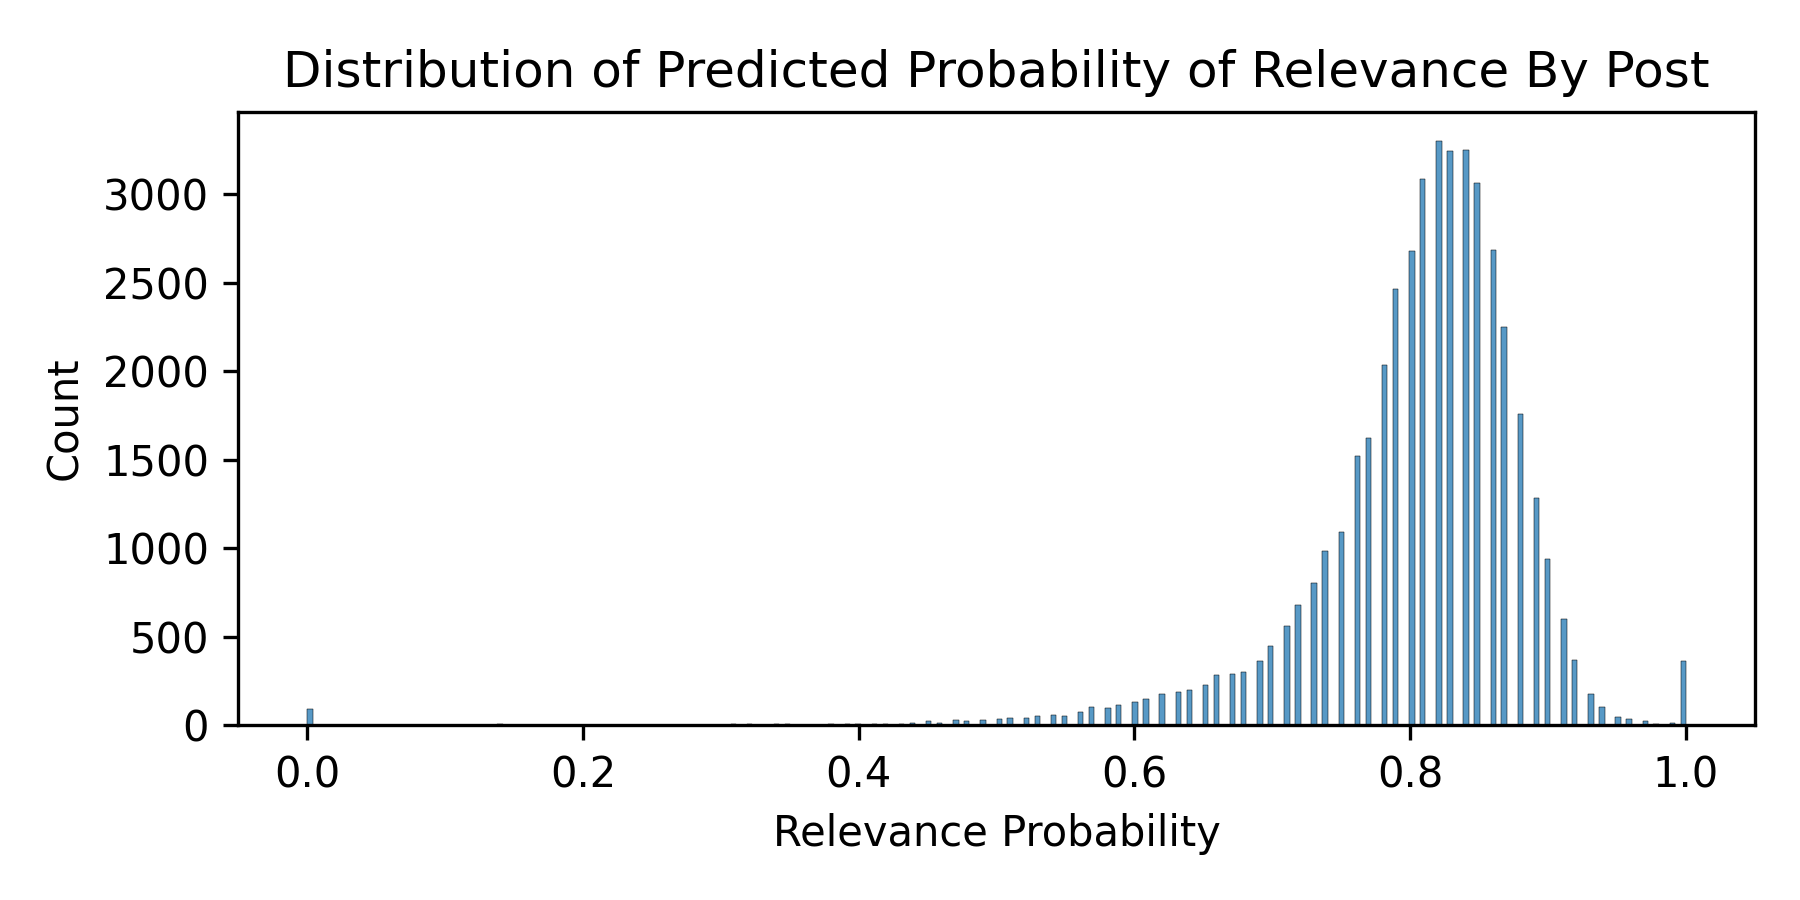
\includegraphics[width=0.8\linewidth, height=0.8\textheight, keepaspectratio]{../../corpus/combined/related_proba_dist.png}
    \caption{Distribution of LR-predicted relevance probability}
    \label{fig:relevance_dist}
\end{figure}

Finally, the data is de-duplicated by \texttt{note\_id} and \texttt{medicine\_name}, resulting in a total of 31,430 entries. This includes 18,038 unique posts (by \texttt{note\_id}), of which 12,806 are from Weibo and 5,232 are from Reddit. As shown in figure \ref{fig:cleanup_posts}, the distribution is quite imbalanced. While substantial numbers of posts mentioning EBM are obtained both from Weibo and Reddit, almost all TCM posts come from Weibo. This distribution is as expected and shows how scarce the discussion on TCM is in English-speaking countries. Although it can be argued that, in some cases (like for Qingshi Antipruritic Ointment), poor keyword choices result in rare matches, this data distribution itself is reflective of the poor recognition of TCM in English-speaking countries.

\begin{figure}[htbp]
    \centering
    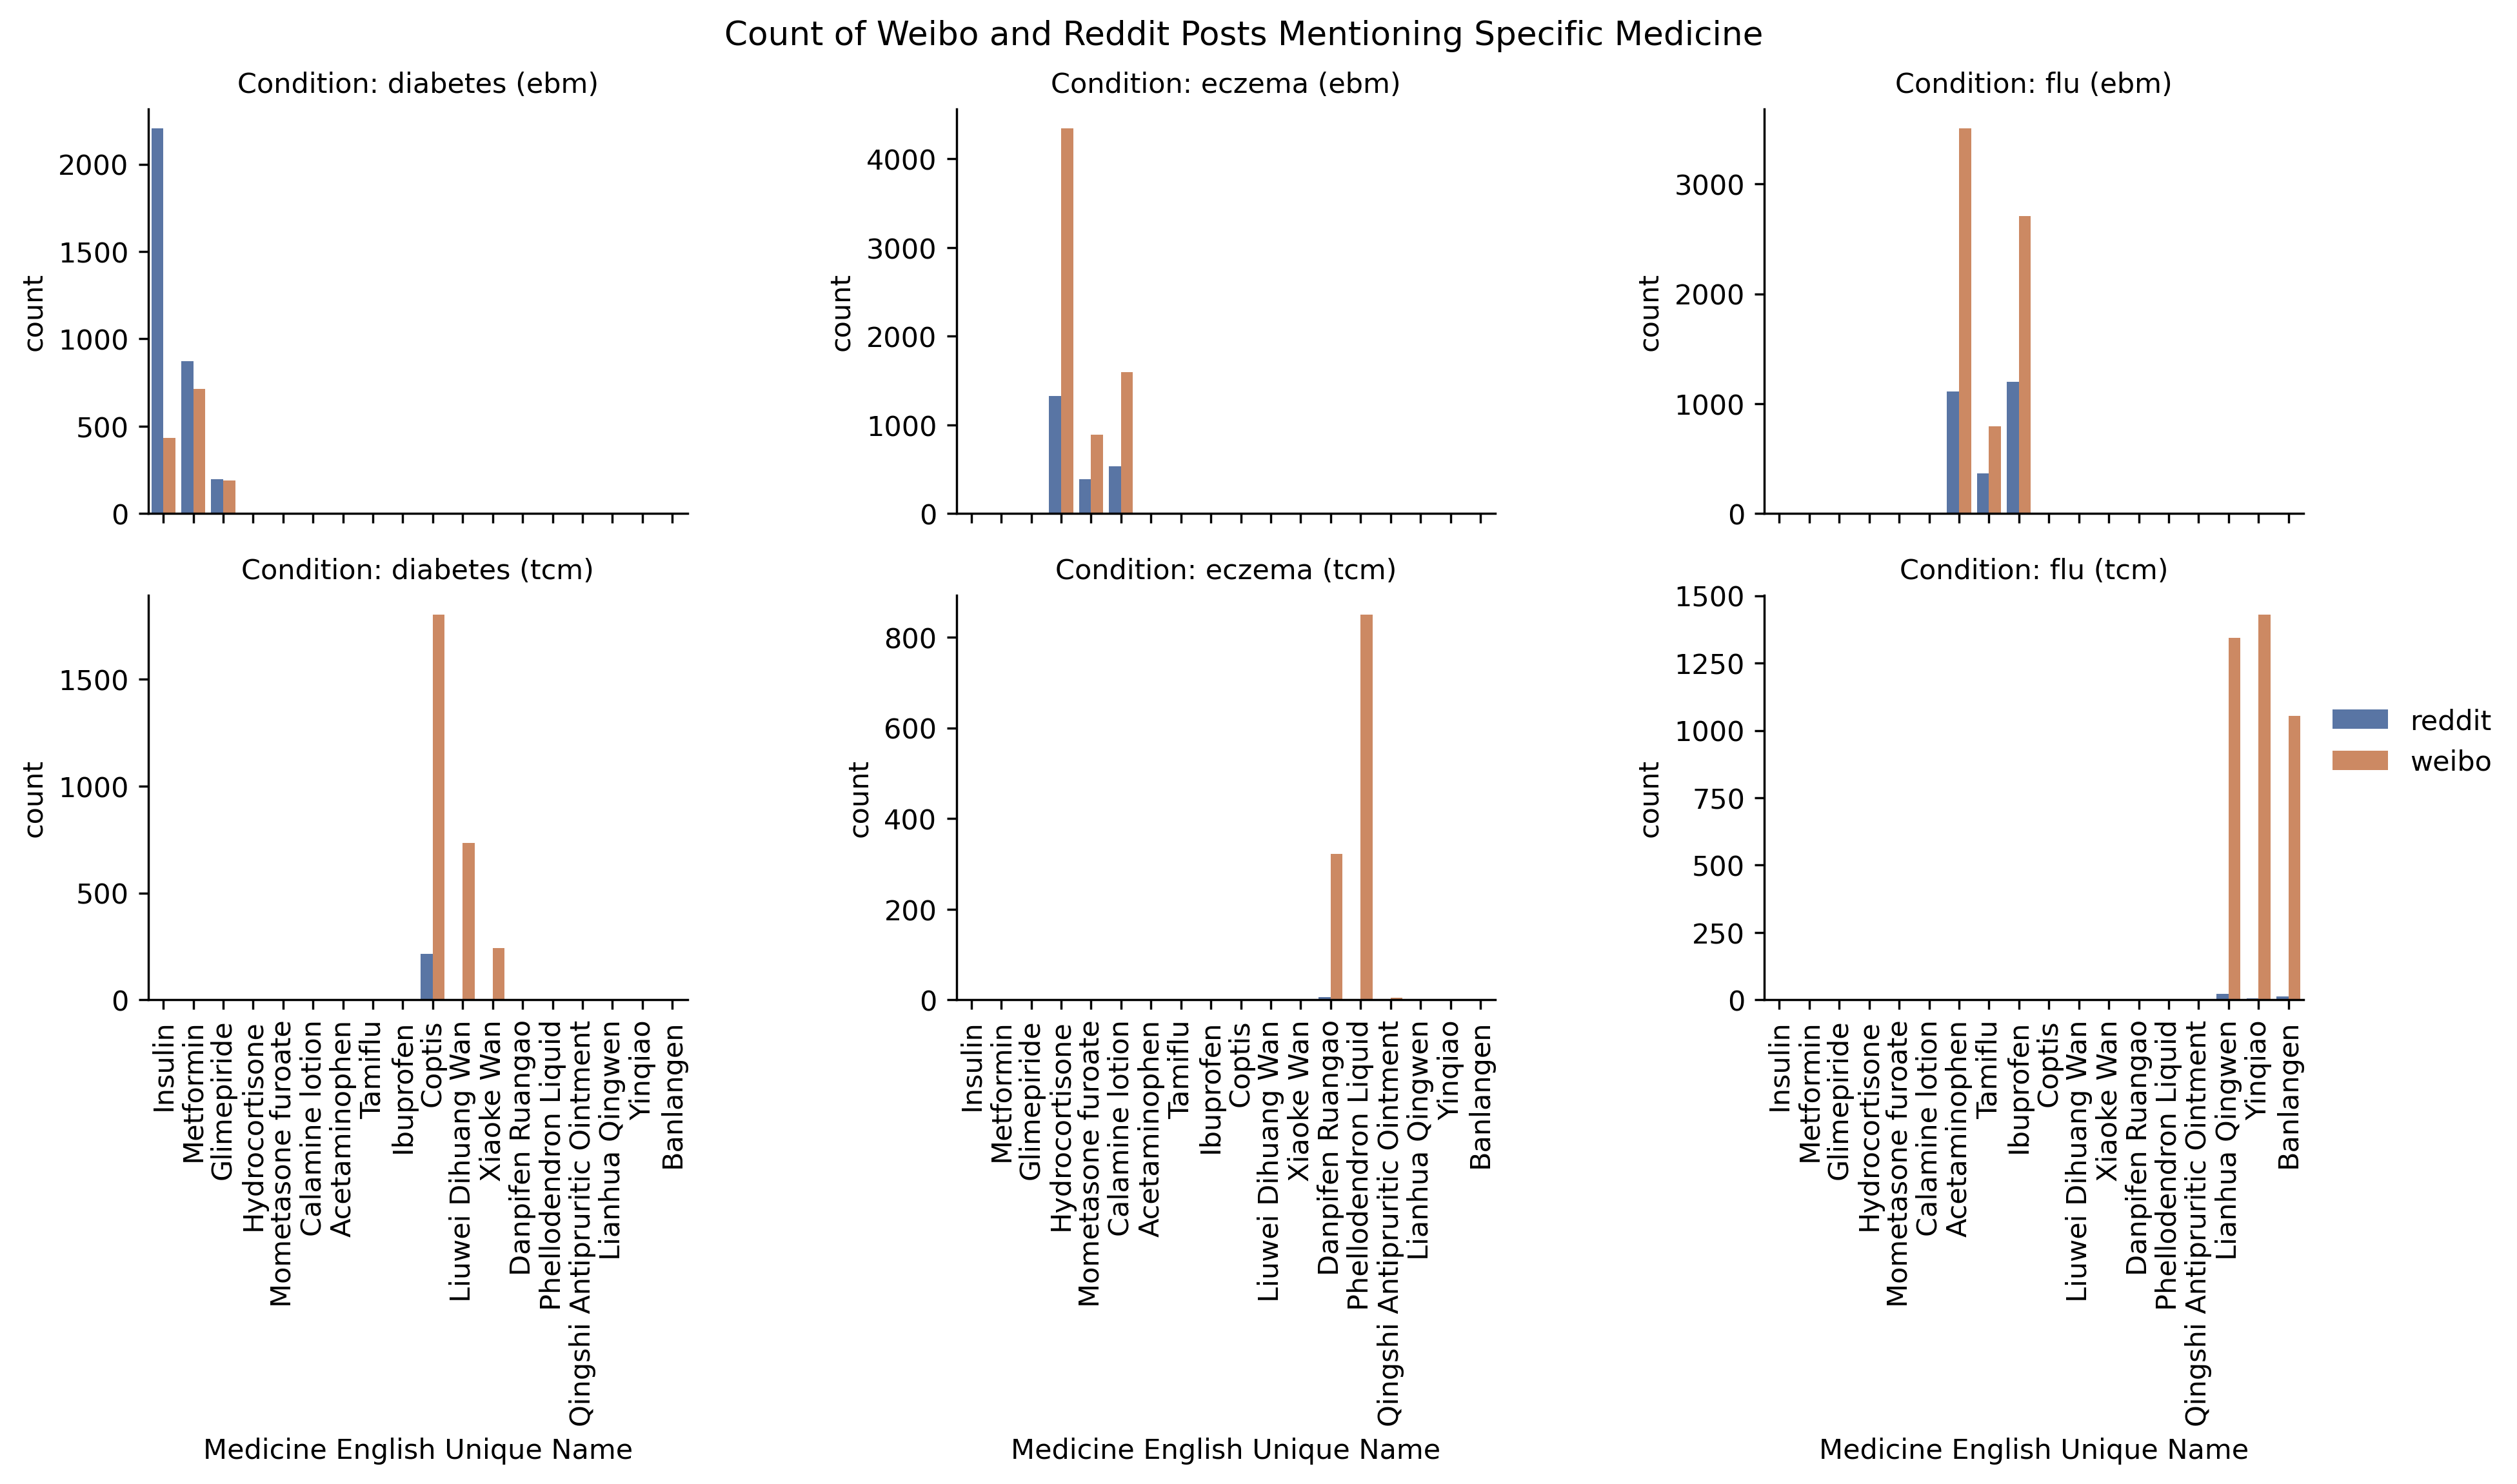
\includegraphics[width=0.8\linewidth, height=0.8\textheight, keepaspectratio]{../../scraping/plots/combined_filtered_counts.png}
    \caption{Distribution of LR-predicted relevance probability}
    \label{fig:cleanup_posts}
\end{figure}

\section{Method}

Opinion mining examines user attitudes toward certain aspects of interest using mass online reviews. Here I define the 18 medicines as the aspects of interest and examine public attitudes toward them using the compiled posts from Reddit and Weibo. My analyses follow three steps: Aspect-Based Sentiment Analysis (ABSA), Machine Learning (ML) classification, and statistical analyses.

\subsection{Aspect-Based Sentiment Analysis (ABSA)}
As \textcite{gao_2021_weibo} found in their study, social media posts are nuanced with emotions not necessarily associated with TCM despite matching the keyword, which can significantly impact the results. ABSA is a fine-grain approach to sentiment analysis that classifies emotions toward an entity \parencite{piedrahitavalds_2021_vaccine}, which minimizes the influence from noisy data by analyzing the sentence components directly related to the aspect.

Extraction of relevant components is performed using pre-trained Chinese and English models with the \texttt{spaCy} package, which tokenize the document and perform part-of-speech (POS) tagging and dependency parsing. Since many of the medicine keywords are phrases that gets broken up during tokenization, a re-tokenization step is introduced to merge each phrase into one token. When one phrase matches multiple keywords (for example, "Lianhua Qingwen Capsule" matches "Lianhua Qingwen" and itself), only the longest combination is kept. Therefore, this step also acts as a second de-duplication step, ensuring the same aspect is not counted twice.

Relevant parts of the sentences are then extracted based on the dependency tree. The entire subtree of the aspect keyword is first extracted, which represent the immediate modifiers of the aspect. The anchor (the closest verb or adjective to the aspect, or the tree root) of the sentence is then identified, and the subtrees of any of its child nodes satisfying the defined dependencies are extracted. The list of dependencies to extract are shown in table \ref{tab:deps}. Three extra dependencies are allowed for Chinese texts, which have fundamentally different linguistic features from English. Chinese characters are not separated by spaces, leading to less predictable tokenization behaviors of the model. This further affects POS and dependency tags, resulting in a larger number of unclassified dependents (dep). These tags are included in the extracted components since they sometimes comprise a large portion of the sentence, and leaving them out can lead to a nonsense result. The auxiliary:aspect tag (aux:asp) includes prevalent state markers in Chinese (examples: "\cn{了}", "\cn{过}"), while adjectival modifiers (amod) include modifier phrases that end with "\cn{的}", which is a common pattern in Chinese.

\begin{table}[htbp]
    \centering
    \renewcommand{\arraystretch}{1.2}
    \begin{tabular}{|l|l|c|c|}
        \hline
        \textbf{Dependency} & \textbf{Description} & \textbf{English} & \textbf{Chinese} \\
        \hline
        \textbf{acomp} & adjectival complement & \checkmark & \checkmark \\
        \hline
        \textbf{advmod} & adverbial modifier & \checkmark & \checkmark \\
        \hline
        \textbf{neg} & negation modifier & \checkmark & \checkmark \\
        \hline
        \textbf{dobj} & direct object & \checkmark & \checkmark \\
        \hline
        \textbf{xcomp} & open clausal complement & \checkmark & \checkmark \\
        \hline
        \textbf{attr} & attribute & \checkmark & \checkmark \\
        \hline
        \textbf{dep} & unclassified dependent & $\times$ & \checkmark \\
        \hline
        \textbf{aux:asp} & auxiliary:aspect & $\times$ & \checkmark \\
        \hline
        \textbf{amod} & adjectival modifier & $\times$ & \checkmark \\
        \hline
    \end{tabular}
    \caption{List of allowed dependencies for the child of the sentence anchor to be included.}
    \label{tab:deps}
\end{table}

Moreover, unlike English, which is a hypotactic language with explicit connectives between clauses, Chinese is highly paratactic that depends on semantics and context to connect the clauses \parencite{mak_2015_parataxis}. This means that many components associated with the target aspect will be buried in separate clauses that are filtered out based on the rules above. As an example, the sentence in figure \ref{fig:absa_example_2} (which directly translates to "when having a fever why take TCM, take Ibuprofen, see effects fast") is seperated into 3 clauses, with the key emotional component "see effects fast" isolated from the aspect "Ibuprofen". To solve this problem, I also included children of the anchor word with dependency labels 'conj' (conjunct), 'parataxis', and 'ccomp' (clausal complement), as well as searching one level up the tree to find clauses that are siblings of the anchor word. This ensures that relevant contexts in Chinese texts can be captured.

\begin{figure}[htbp]
    \centering
    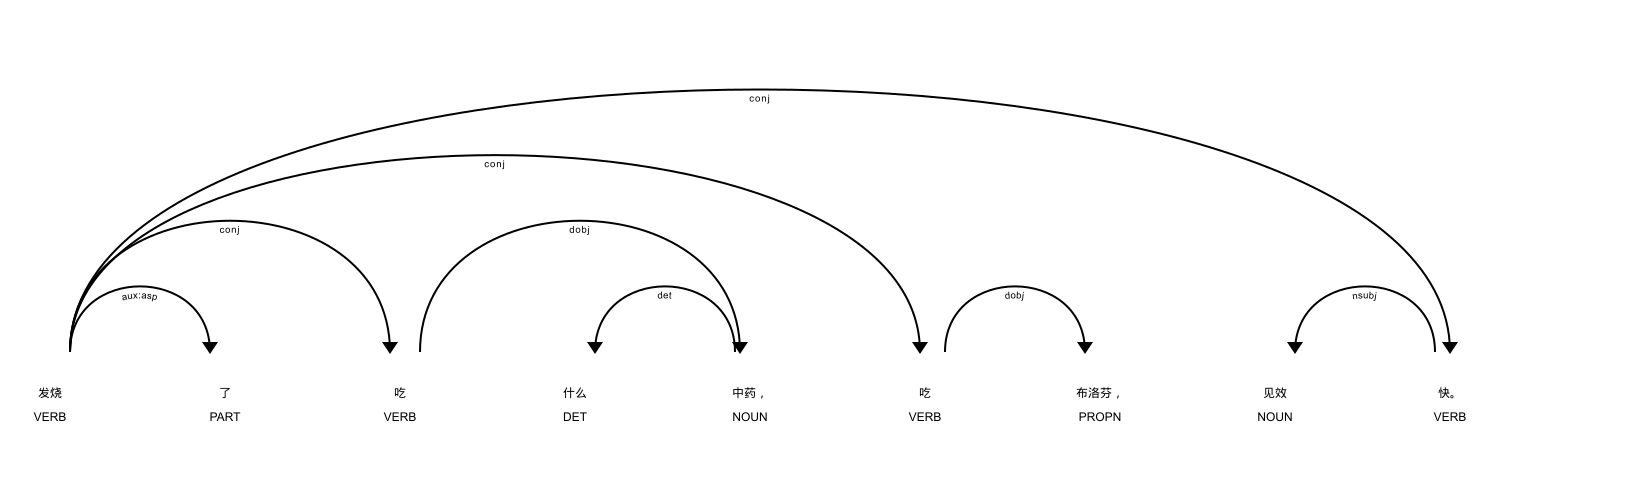
\includegraphics[width=\linewidth, keepaspectratio]{../../results/absa_example_2.png}
    \caption{Dependency parsing example showing the paratactic nature of Chinese.}
    \label{fig:absa_example_2}
\end{figure}

After extraction, the selected tokens are sorted based on their original index and recombined into a pruned sentence. This rule-based aspect extraction approach reliably separates the components of the sentence related to the aspect. Using as an example the sentence "To be honest, the Paeonol cream was not very effective for my back, but the doctors offering it were so sweet." (figure \ref{fig:absa_example}), a sentence-level sentiment analyzer will take in "not effective" as well as "so sweet", which counter each other and result in a neutral sentiment. However, the English parser identifies "was" as the anchor, includes the adjectival complement "effective" while discarding the second half of the sentence completely by filtering out the conjunct "were", resulting in the pruned sentence "the Paeonol cream was not very effective for my back."

\begin{figure}[htbp]
    \centering
    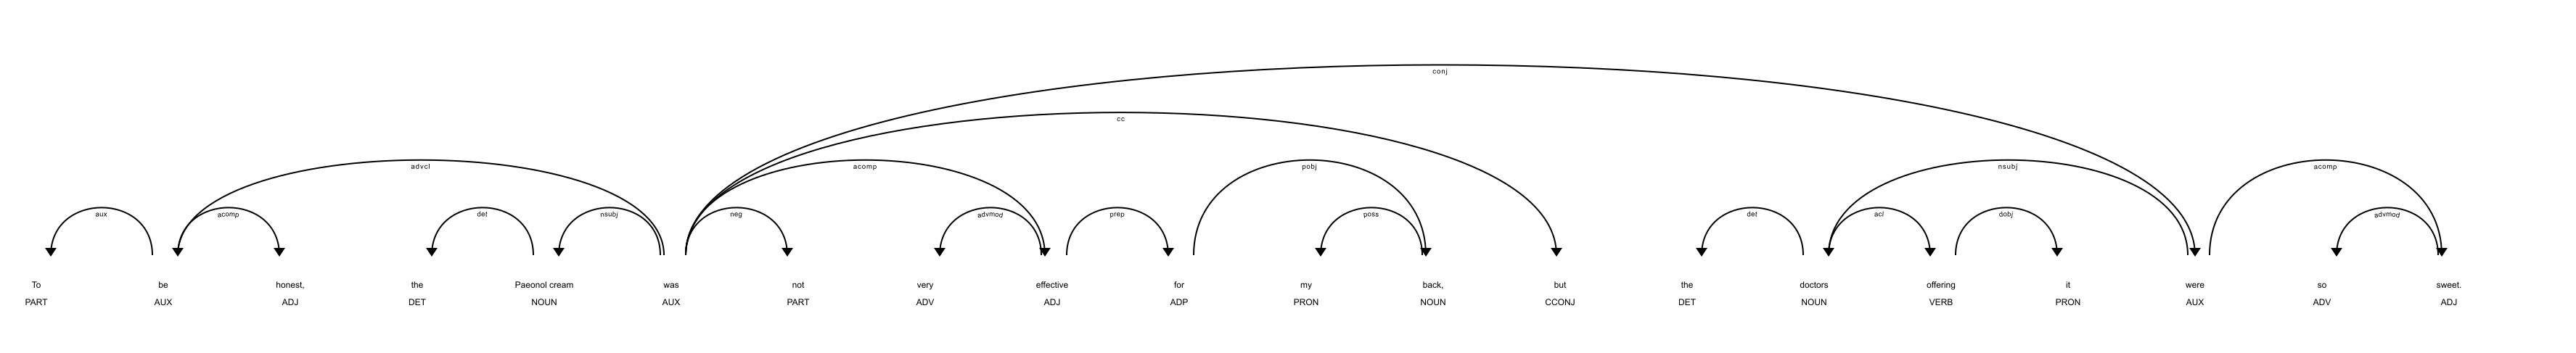
\includegraphics[width=\linewidth, keepaspectratio]{../../results/absa_example.png}
    \caption{Dependency parsing example of a noisy sentence.}
    \label{fig:absa_example}
\end{figure}

After aspect extraction, sentiment analysis is performed using straightforward models. The Valence Aware Dictionary and sEntiment Reasoner (VADER) lexicon is used with Natural Language Toolkit (NLTK) to analyze English texts, while SnowNLP is employed for Chinese sentiment analysis which is based on a naive Bayesian classifier. VADER compound scores are used, which are within the range of [-1, 1]. They are then classified into positive ($> 0.05$), neutral ($-0.05 < s \leq 0.05$), or negative ($\leq -0.05$), following the recommendations of the package authors, and further normalized to a range of [0, 1]. SnowNLP outputs probabilities of the text being positive in the range of [0, 1]. A conventional equal threshold is applied to classify them as positive ($>0.66$), neutral ($0.33 < s \leq 0.66$), or negative ($\leq 0.33$). Since the scores are generated using different pruning strategies and different sentiment analysis methods, they are not directly comparable to each other. Statistical tests in the following sections will aim to compare within languages.

\subsection{Machine Learning (ML) Trust Classification}

Although ABSA reduces noise of the data, sentiment is not a perfect proxy for trust. Take the following ABSA-cleaned Chinese post as an example: "\cn{疼腰疼十一点多吃的对乙酰氨基酚片但还是疼，受不了了刚刚又吃了一颗不知道能不能再缓解一点}" (My lower back hurts. I took Acetaminophen a little after 11, but it still hurts. I can't stand it anymore, so I just took another one.  I don't know if it will relieve it a bit more.) This sentence will be classified as strongly negative by any sentiment analyzer, but it in fact signifies strong trust in Acetaminophen since the poster relies on it for pain control.

The large-size XLM-RoBERTa model \parencite{DBLP:journals/corr/abs-1911-02116} is fine-tuned to classify the posts into either trust, neutral or distrust towards the target aspects. A random sample of 637 posts, stratified by language, is manually annotated and used to train the classifier. Early stopping is applied to prevent overfitting, and validation loss was minimum at epoch 15. This labeled set is further split into 80\% training set and 20\% validation. Using a linear classification head with a dropout of 50\%, the model achieved a high recall of 78\% with a lower precision of 69\% after adjusting for the weights of different prediction classes, with a high ROC-AUC of 0.91 showing its discriminatory power (table \ref{tab:trust_stats}). Since the performance metrics are macro-averages, they are heavily influenced by predictions of class labels with the fewest number of entries (which is distrust). The F1 score takes into account both precision and accuracy, and a macro-average F1 score of 0.70 for a 3-class predictor indicates solid performance.

\begin{table}[htbp]
    \centering
    \renewcommand{\arraystretch}{1.5}
    \begin{tabular}{|l|l|l|l|l|l|}
        \hline
        \textbf{} & \textbf{Precision} & \textbf{Recall} & \textbf{Accuracy} & \textbf{F1 Score} & \textbf{ROC-AUC} \\
        \hline
        \textbf{Raw Predictions} & 0.64 & 0.75 & 0.66 & 0.63 & 0.90 \\
        \hline
        \textbf{Weight Adjusted} & 0.69 & 0.78 & 0.73 & 0.70 & 0.91 \\
        \hline
    \end{tabular}
    \caption{Macro averages of trust classifier performance on the validation set.}
    \label{tab:trust_stats}
\end{table}

The model is re-trained on the entire labeled set with a hard stop at 15 iterations to prevent overfitting. It is then applied to classify the whole dataset.

\subsection{Statistical Analyses}

Both ABSA and ML results are aggregated based on their publishing time, with COVID period defined as publishing time between year 2019 and 2023 and post-COVID as year 2024 and after. Statistical tests are performed on both the ABSA and ML results to answer each of the three comparative questions. To account for community consensus and visibility, each analysis is performed first on post counts and then repeated using data weighteed by user upvotes. All tests are performed at a significance level of $\alpha=0.05$ with Bonferroni correction to control for false positive rates during multiple comparisons.
\begin{enumerate}
    \item \textbf{Temporal Shifts:} Is there a difference between COVID and post-COVID opinions on the same types of medicines?
    \begin{itemize}
        \item \textbf{Post Count:} A two-sample, two-tailed z-test is performed on each type of medicine on each platform, comparing the proportion of positive/trustful posts during and post-COVID.
        \item \textbf{Upvote Weighted:} A permutational test is performed by randomly shuffling time period labels 999 times. The empirical difference in upvote-weighted proportions of positive/trustful posts during and post-COVID is compared to the null distribution to establish a two-tailed p-value.
    \end{itemize}

    \item \textbf{Medicine Types:} Is there a difference between post-COVID opinions regarding EBM vs. TCM?
    \begin{itemize}
        \item \textbf{Post Count:} A two-sample, two-tailed z-test is performed on post-COVID posts on each platform, comparing the proportion of positive/trustful posts on TCM versus EBM.
        \item \textbf{Upvote Weighted:} A permutational test is performed by randomly shuffling medicine type labels 999 times. The empirical difference in upvote-weighted proportions of positive/trustful posts on TCM versus EBM is compared to the null distribution to establish a two-tailed p-value.
    \end{itemize}

    \item \textbf{Geocultural Preferences:} Is there a difference between post-COVID preferences for TCM on Weibo vs. Reddit?
    \begin{itemize}
        \item \textbf{Post Count:} First, a Chi-square test is used to determine if the ratio of TCM to EBM posts, specifically post-COVID posts expressing positive or trustful sentiments, differs between Weibo and Reddit. A permutational difference-in-differences (DiD) test is then conducted by shuffling platform labels 999 times. This allowed the assessment of whether the cross-platform difference in the proportion of these positive/trustful posts post-COVID varied significantly between TCM and EBM.
        \item \textbf{Upvote Weighted:} First, a permutation test is performed by shuffling platform labels 999 times to determine if the upvote-weighted ratio differs between Weibo and Reddit. Then, a permutational DiD test is conducted similarly for upvote-weighted proportions as for post counts.
    \end{itemize}
    
\end{enumerate}

\section{Results}

\subsection{Overview}

After ABSA-extraction and filtering out rows with no aspect matches, 26,848 entries remain and are used in statistical analyses. The post numbers for different medicine types and categories are shown by platform in figure \ref{fig:count}. It should be noted that, while TCM posts are in general scarce on Reddit, the number of posts for TCM eczema medicines and the number of post-COVID posts for TCM flu medicines are especially small, which negatively impacts the soundness of the statistical analyses.

\begin{figure}[htbp]
    \centering
    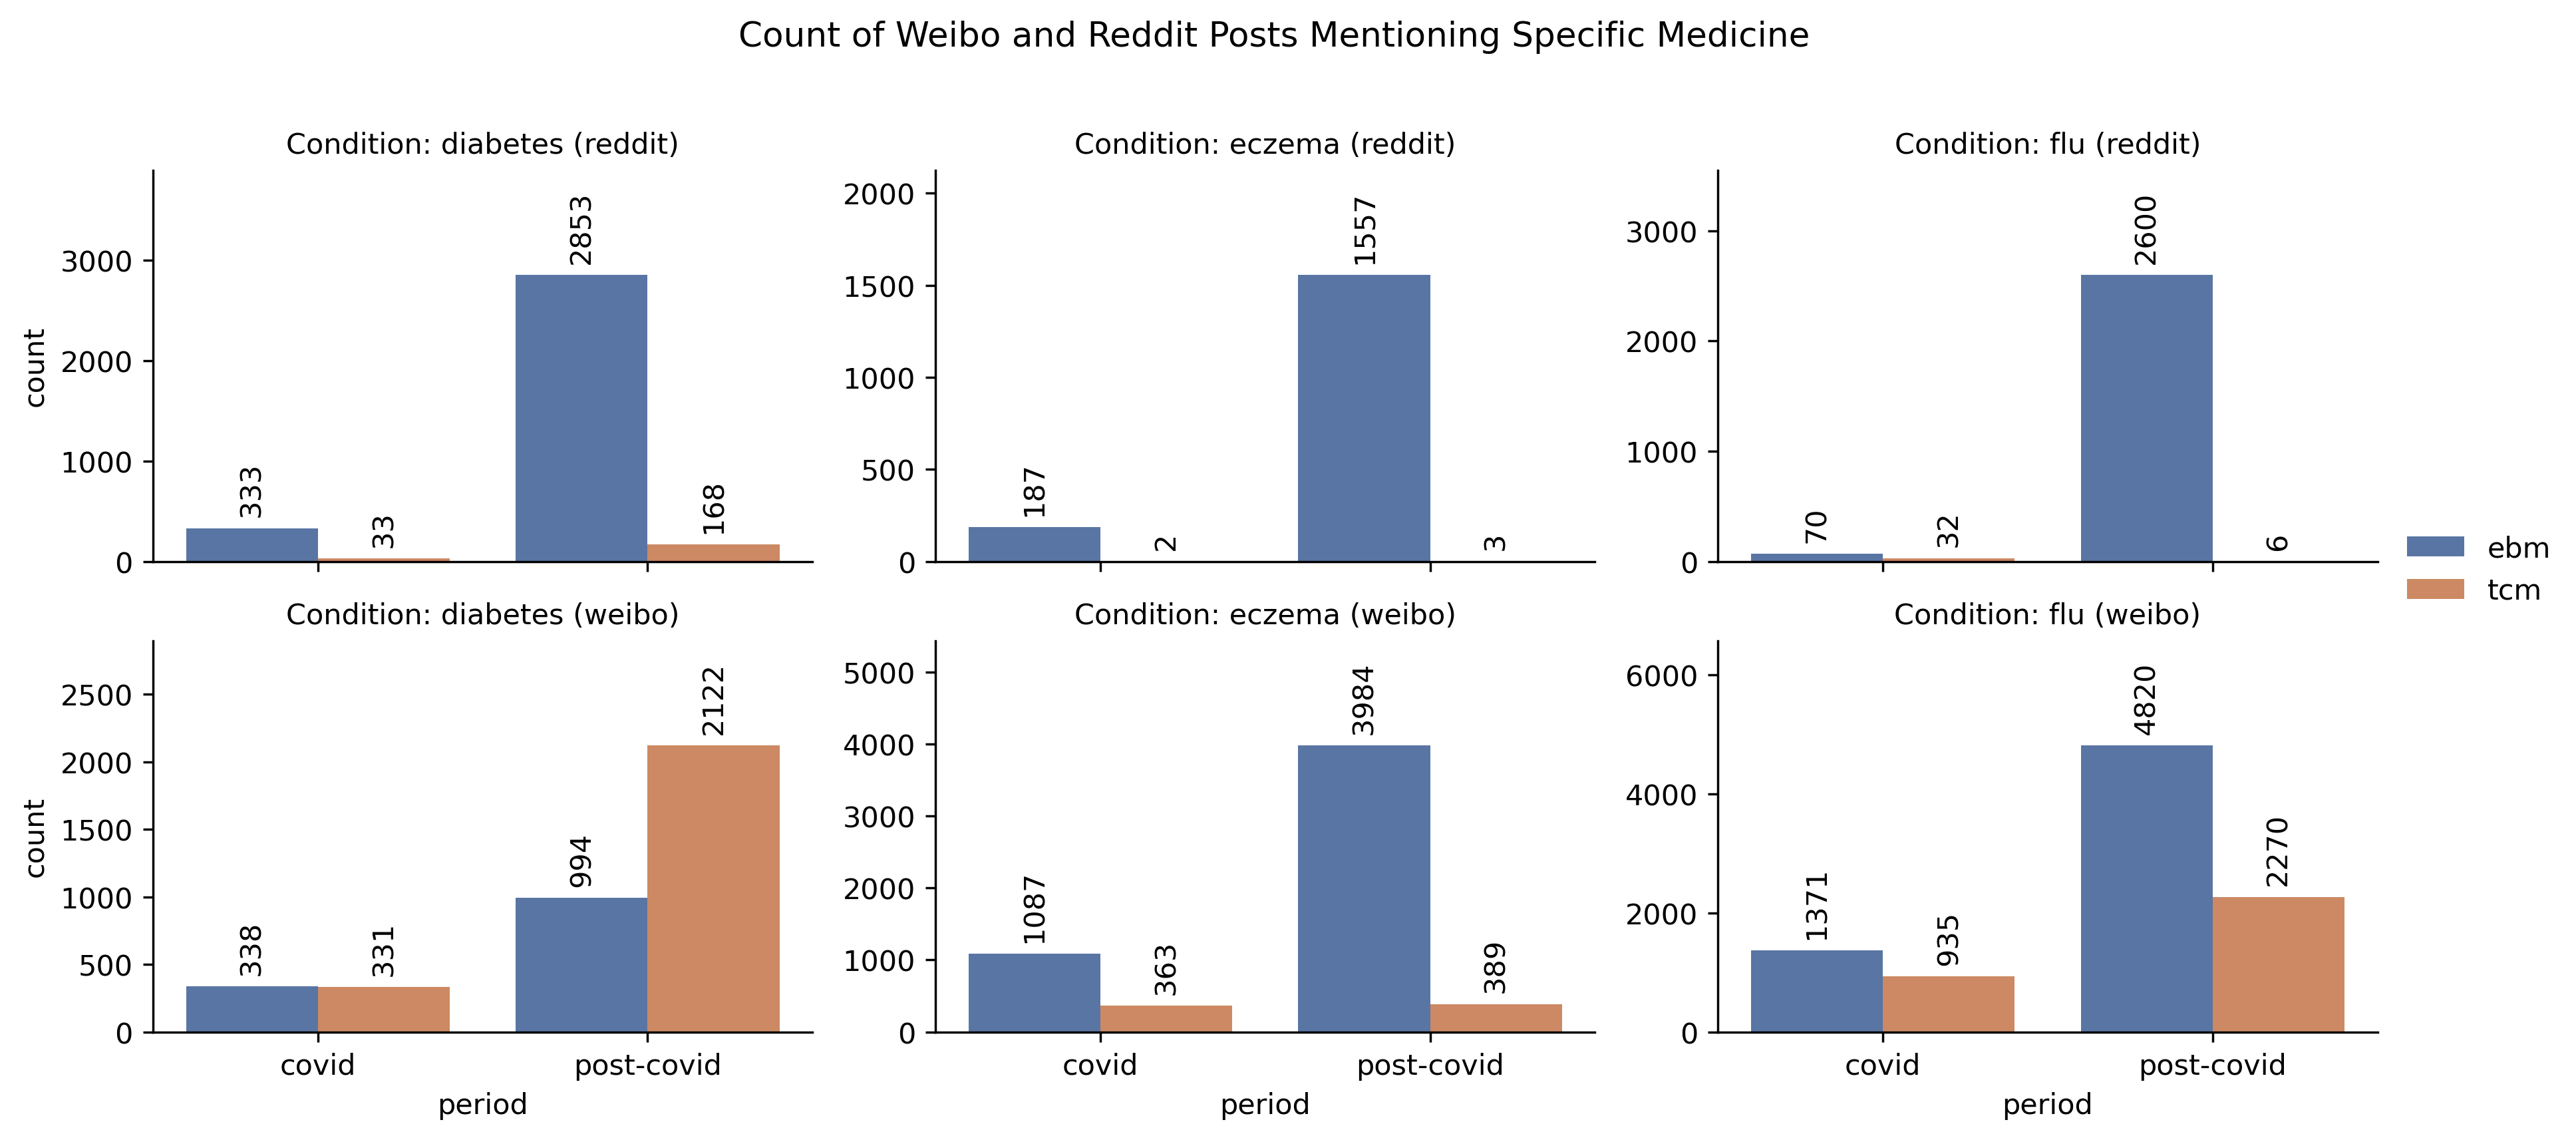
\includegraphics[width=0.8\linewidth, keepaspectratio]{../../results/absa_count_labeled_by_period.png}
    \caption{Number of ABSA-extracted posts by medicine type, medicine category and time period}
    \label{fig:count}
\end{figure}

\subsection{ABSA}

Figure \ref{fig:absa} shows the average normalized sentiment scores by medicine type and category for different platforms across time, with the shaded areas representing 95\% confidence intervals. Unlike EBM which shows a generally stable trend across the time period examined, sentiments on TCM experience large fluctuations at year 2021 (pandemic peak) on Weibo and year 2024 (just after the pandemic) on Reddit. Directly reading off the graph, we see overall similarly neutral attitudes toward both TCM and EBM on Reddit, while sentiments on Weibo exhibit a more interesting difference. Attitudes toward TCM medicines for diabetes and eczema are overall less positive than those toward EBM, but this relationship flips for flu medicines. When weighted by upvotes, as shown in Figure \ref{fig:weighted_absa}, the trend on Reddit remain unchanged, but the fluctuations in the overall sentiments on Weibo are amplified. Weibo attitudes toward TCM and EBM follow more closely when weighted by upvotes, although there is a lower trend in sentiment towards TCM diabetes medicines compared to EBM.

\begin{figure}[htbp]
    \centering
    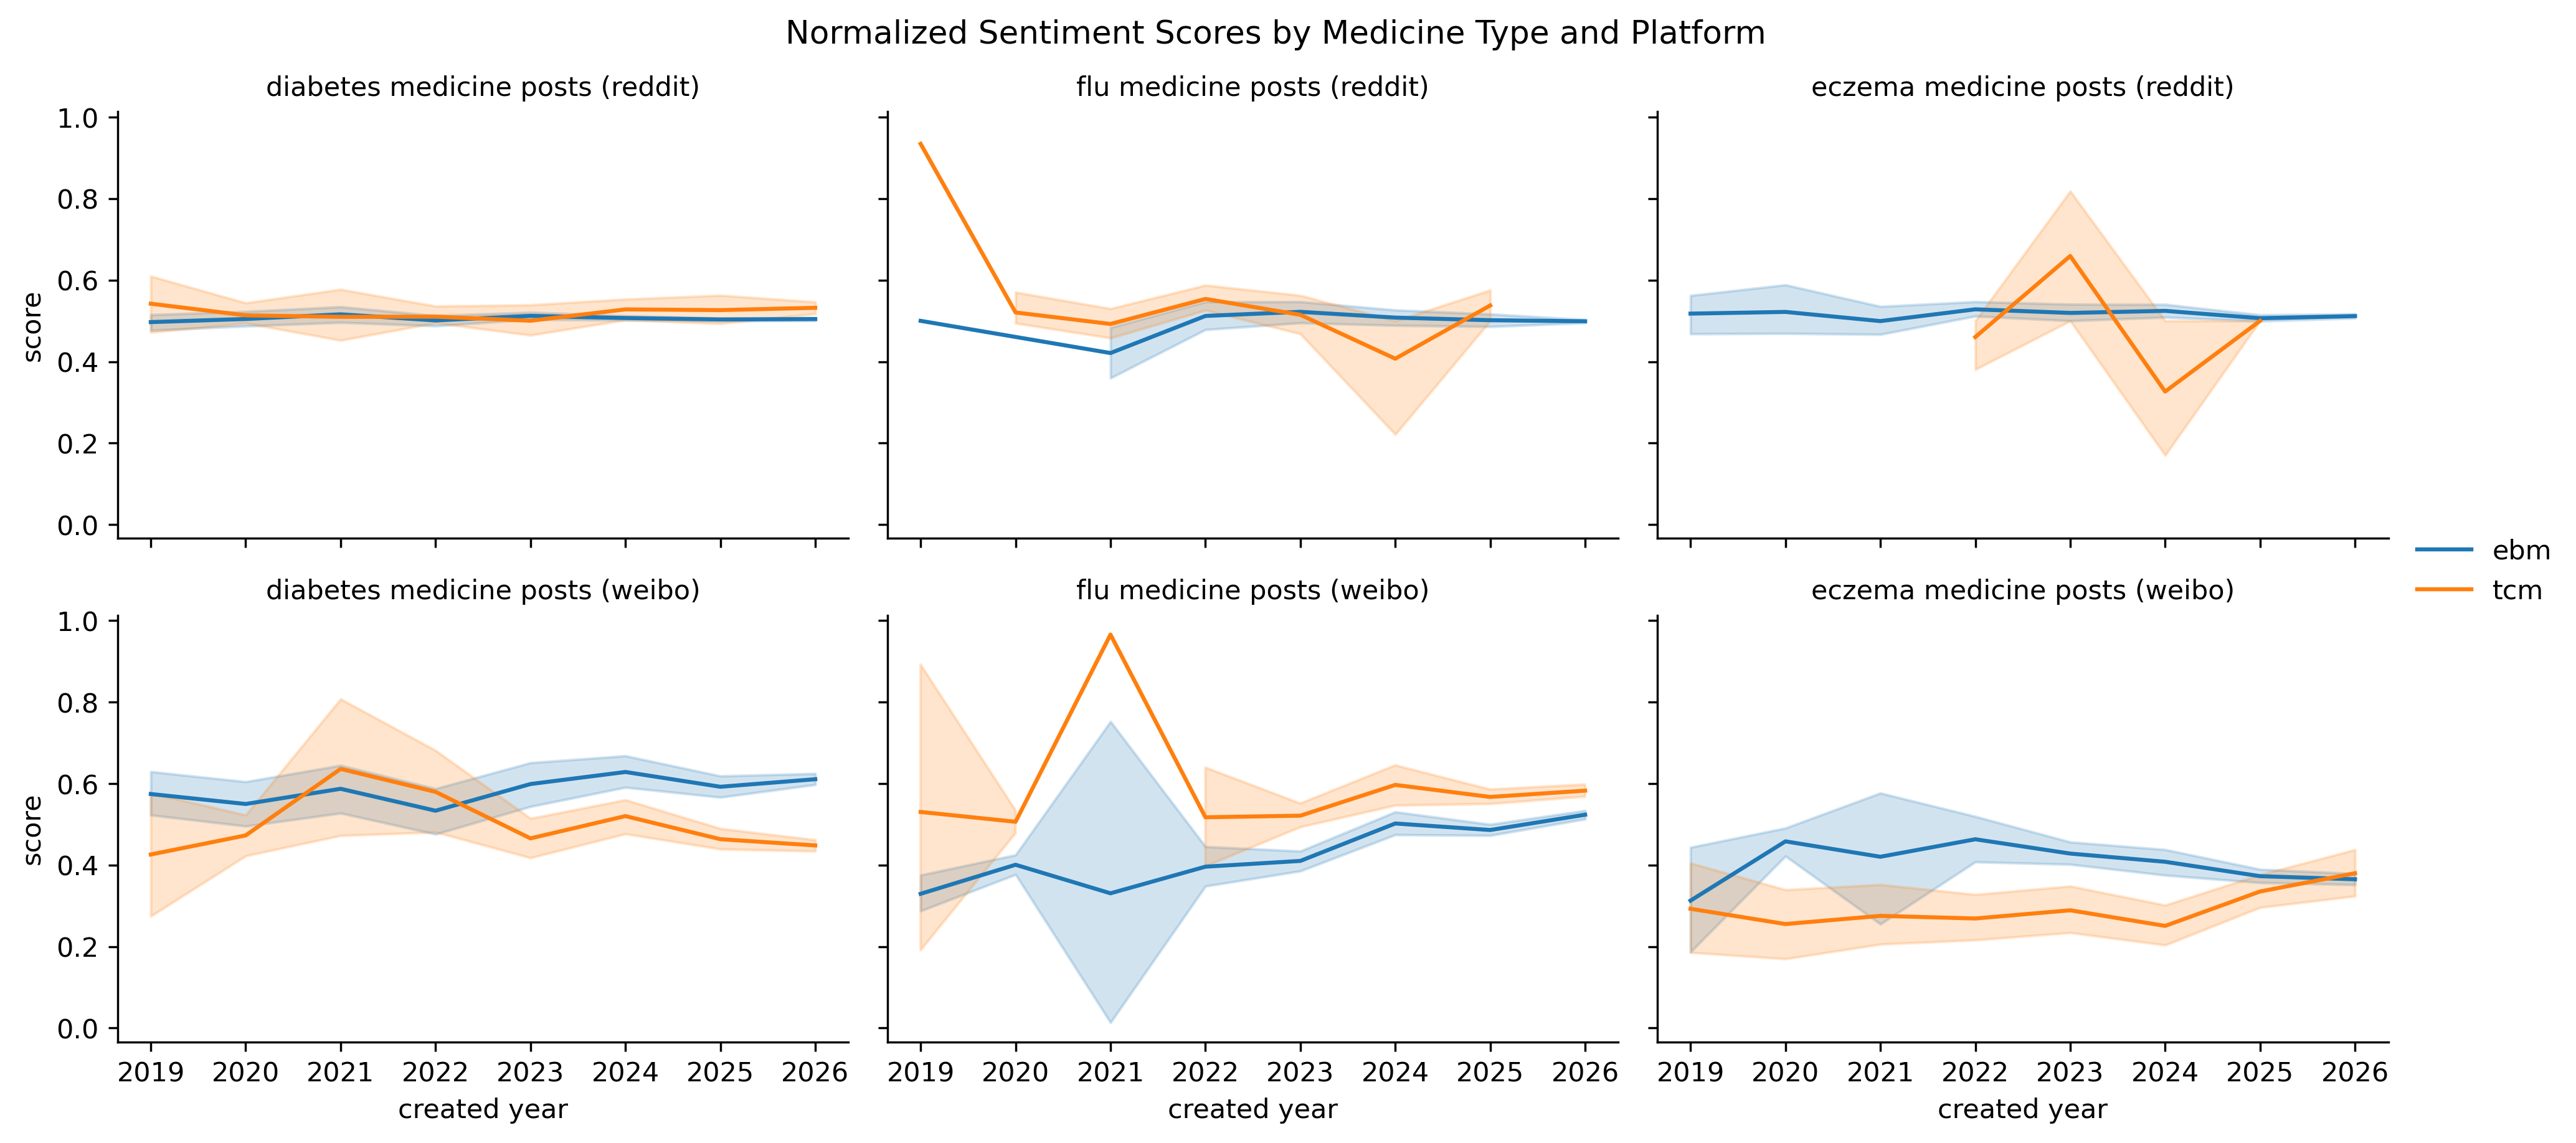
\includegraphics[width=0.8\linewidth, keepaspectratio]{../../results/absa_scores.png}
    \caption{Average ABSA sentiment scores by medicine type and platform. Shaded areas show 95\% confidence intervals.}
    \label{fig:absa}
\end{figure}

\begin{figure}[htbp]
    \centering
    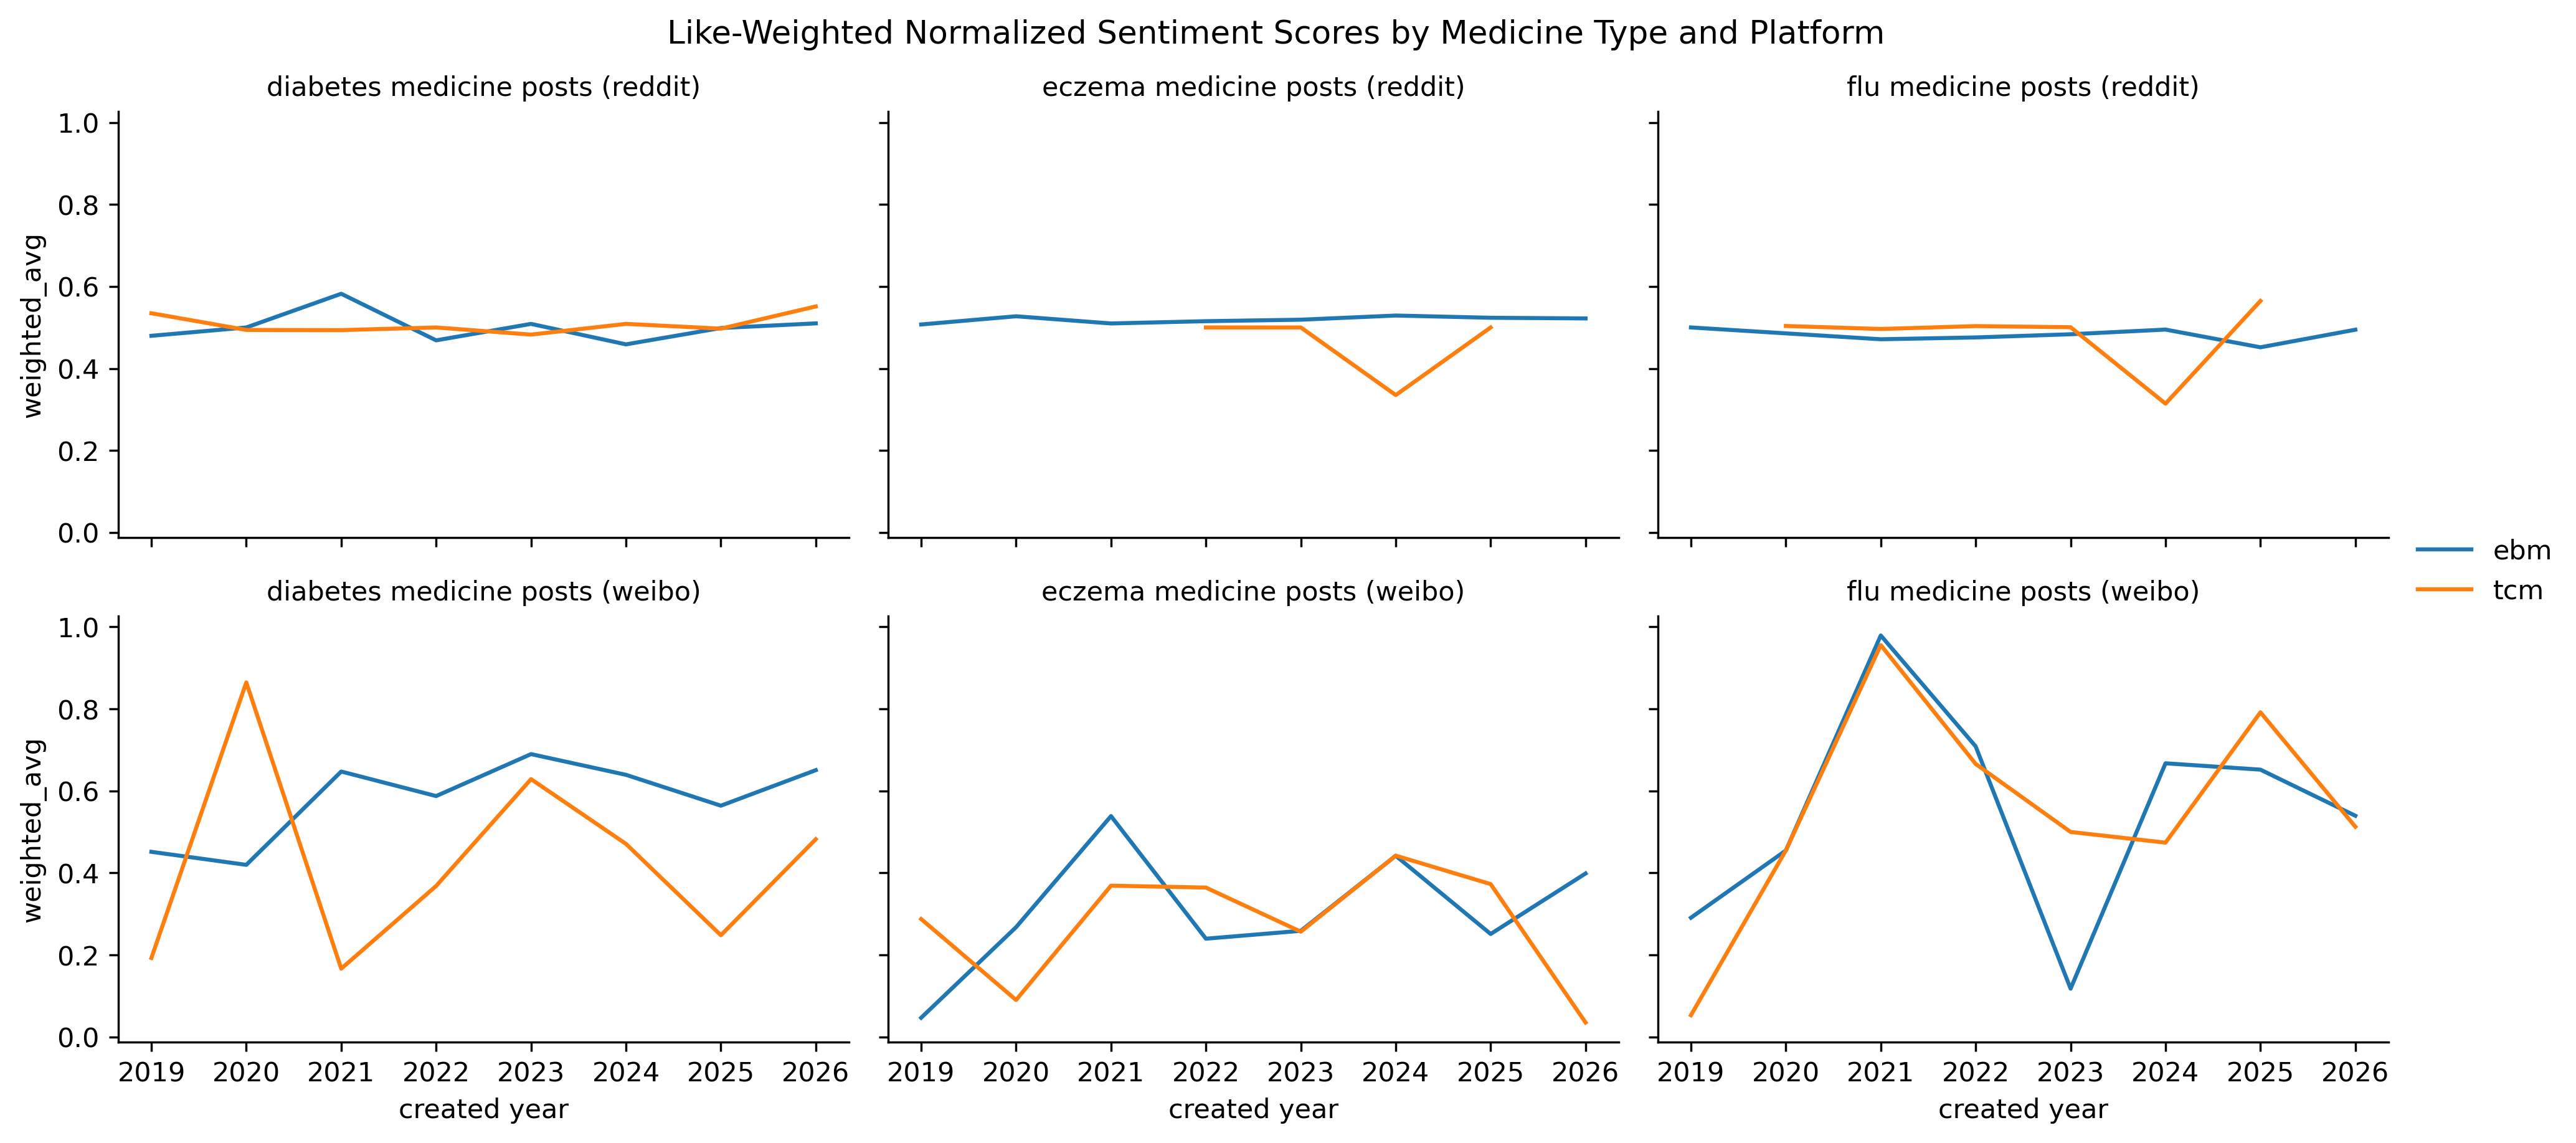
\includegraphics[width=0.8\linewidth, keepaspectratio]{../../results/absa_scores_weighted.png}
    \caption{Upvote-weighted average ABSA sentiment scores by medicine type and platform.}
    \label{fig:weighted_absa}
\end{figure}

\begin{figure}[htbp]
    \centering
    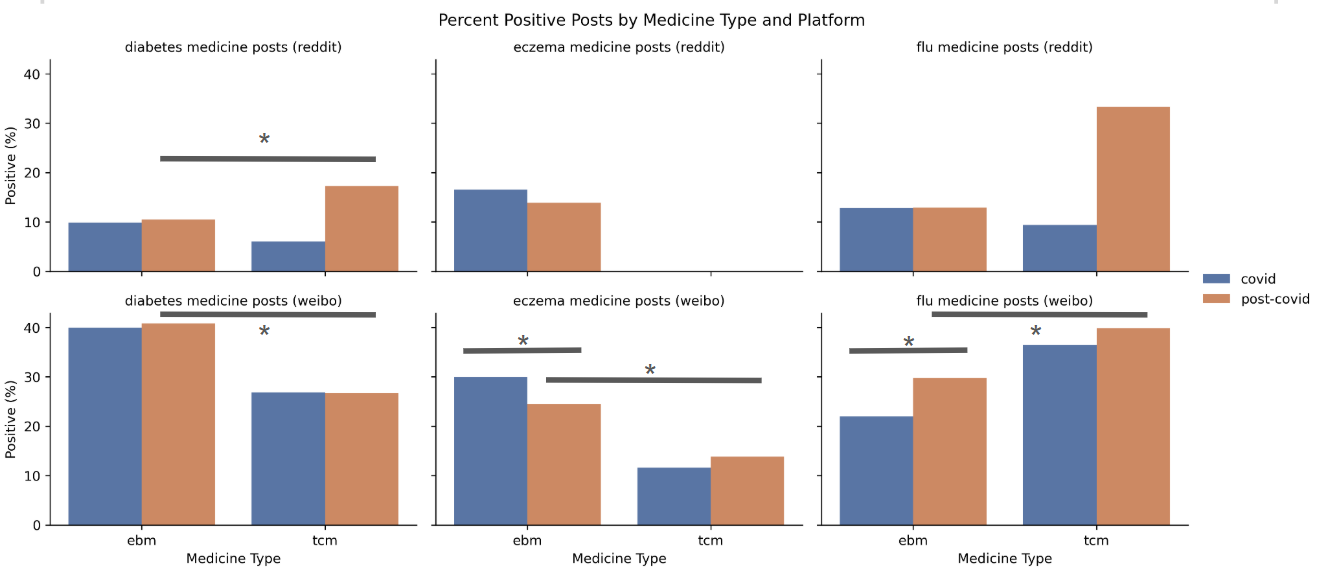
\includegraphics[width=0.8\linewidth, keepaspectratio]{../../results/within.png}
    \caption{Percent positive posts by medicine type and platform, with siginificant within-platform differences labeled.}
    \label{fig:absa_within}
\end{figure}

\begin{figure}[htbp]
    \centering
    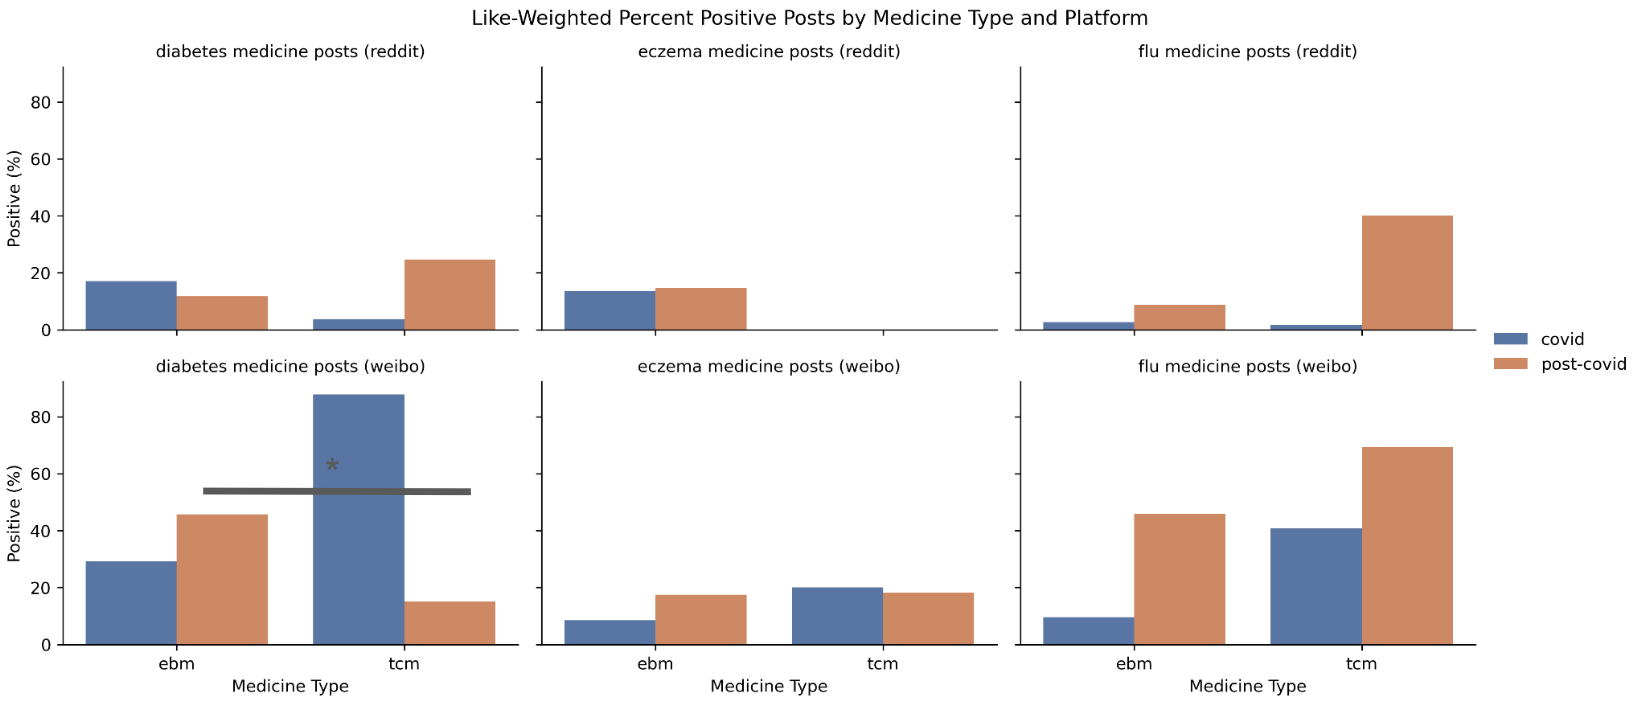
\includegraphics[width=0.8\linewidth, keepaspectratio]{../../results/like_weighted_within.png}
    \caption{Upvote-weighted percent positive posts by medicine type and platform, with siginificant within-platform differences labeled.}
    \label{fig:weighted_absa_within}
\end{figure}

\begin{figure}[htbp]
    \centering
    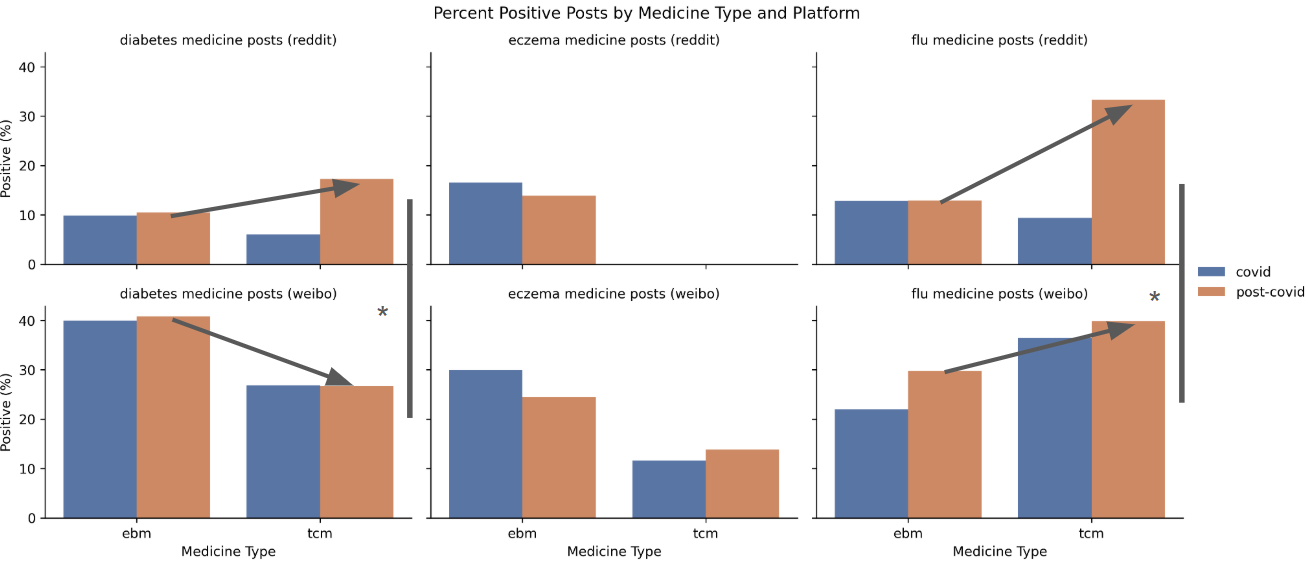
\includegraphics[width=0.8\linewidth, keepaspectratio]{../../results/between.png}
    \caption{Percent positive posts by medicine type and platform, with siginificant between-platform differences labeled.}
    \label{fig:absa_between}
\end{figure}

\begin{figure}[htbp]
    \centering
    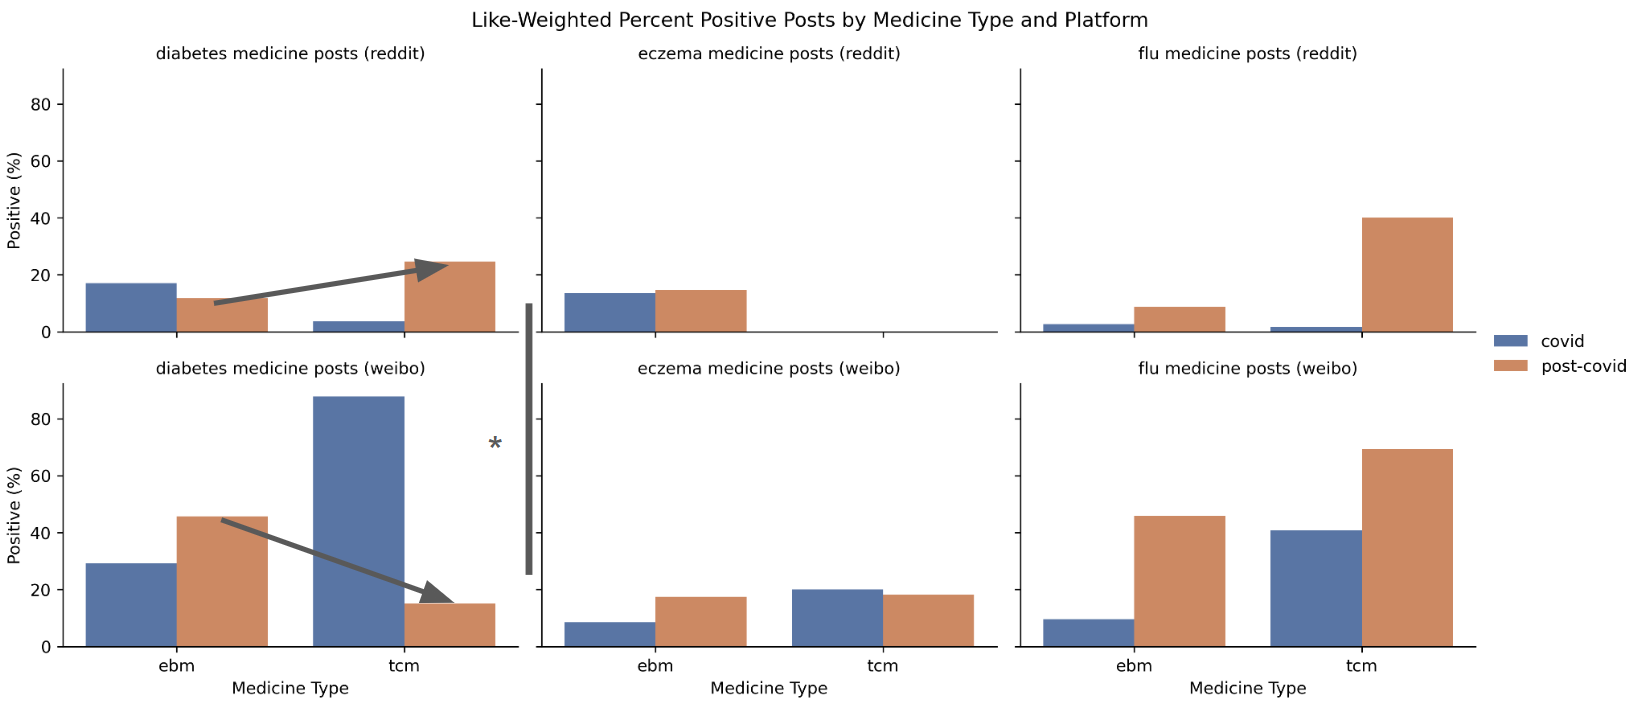
\includegraphics[width=0.8\linewidth, keepaspectratio]{../../results/like_weighted_between.png}
    \caption{Upvote-weighted percent positive posts by medicine type and platform, with siginificant between-platform differences labeled.}
    \label{fig:weighted_absa_between}
\end{figure}

\subsection{ML Classification}

\begin{figure}[htbp]
    \centering
    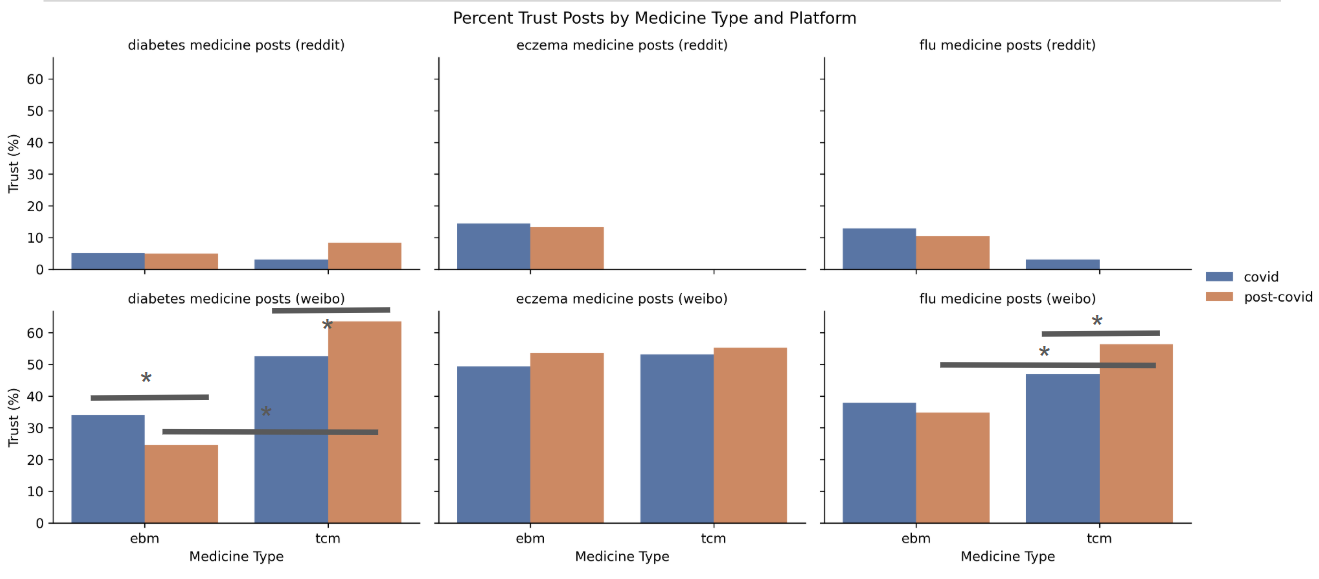
\includegraphics[width=0.8\linewidth, keepaspectratio]{../../results/ml/trust_within.png}
    \caption{Percent trustful posts by medicine type and platform, with siginificant within-platform differences labeled.}
    \label{fig:ml_within}
\end{figure}

\begin{figure}[htbp]
    \centering
    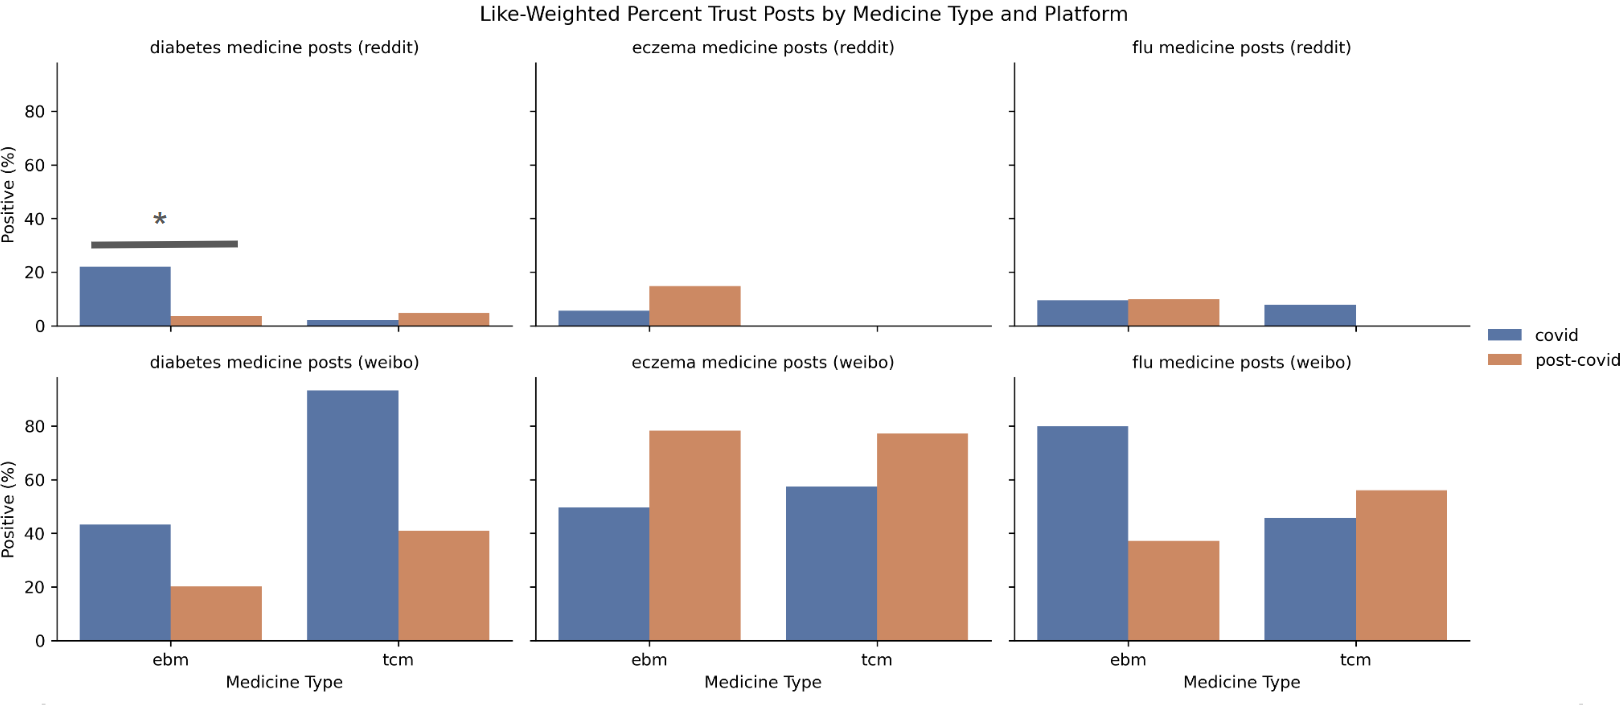
\includegraphics[width=0.8\linewidth, keepaspectratio]{../../results/ml/like_weighted_trust_within.png}
    \caption{Upvote-weighted percent trustful posts by medicine type and platform, with siginificant within-platform differences labeled.}
    \label{fig:weighted_absa_within}
\end{figure}

\begin{figure}[htbp]
    \centering
    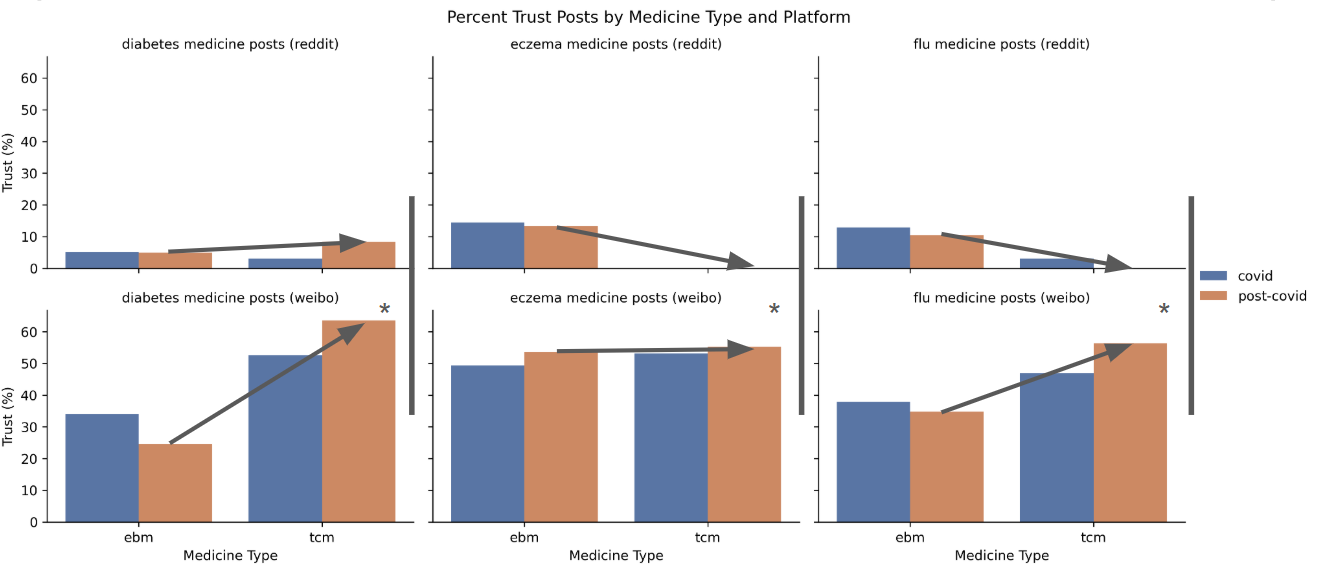
\includegraphics[width=0.8\linewidth, keepaspectratio]{../../results/ml/trust_between.png}
    \caption{Percent trustful posts by medicine type and platform, with siginificant between-platform differences labeled.}
    \label{fig:ml_between}
\end{figure}

\printbibliography[heading=centeredbib, title={References}]


\end{document}